%!TEX root = documentation.tex

\chapter{Introduction}

\section{Project idea}
The idea to this project came up when I was flying my model helicopter. I was wondering how nasty the wind was these days and that it would have been better not to take off into the skies.

But where should I know the conditions from? The wind speed is always different than the values provided by online weather services.\\
That was the point I decided to build something on our own, submitting all the weather data to our website so one can decide beforehand wether to drive to our airfield or not.

\section{Available products on the market}
Having a look on the internet reveals that there are plenty of weather stations available. Nearly all of them provide the basic features like temperature and pressure and a LCD for presenting the current conditions and/or a small forecast.

Some more expensive devices even provide a wind sensor and can be connected to a computer via USB cable. The software shipped with these devices also supports uploading of this data to a website.

So why spending so much time for creating your own product?\\
Comparing the specifications of the wind speed sensors for instance reveals that these very cheap sensors only have limited quality. Also detecting the wind direction was not available in most products, which is essential for airfield applications.\\
Another thing is extensibility, we needed a system that can be extended by new sensors easily and that is flexible enough to generate graphs and diagrams as we like.

The result of this research process was this project called Flight Weather Station (abbr. FWS).

\section{About FWS} % (fold)
\label{sec:about_fws}

As depicted in figure~\ref{fig:overview} FWS consists of the following parts:
\begin{itemize}
\item Sensors: These sensors capture the parameters: Wind speed, wind direction, temperature. Data are transmitted via cable.
\item Controller Board: The controller board collects and processes the data from the sensors and transmits them to the analysis software via Ethernet LAN.
\item Analysis (Software): This software collects the processed data of the Controller Board and performs statistical analysis. It generates diagrams and graphs which are sent to the webserver by a separate script.
\item Webserver (Presentation): The generated diagrams are integrated into the website with a special plugin for the CMS TYPO3.
\end{itemize}

\begin{figure}[ht]
    \centering
    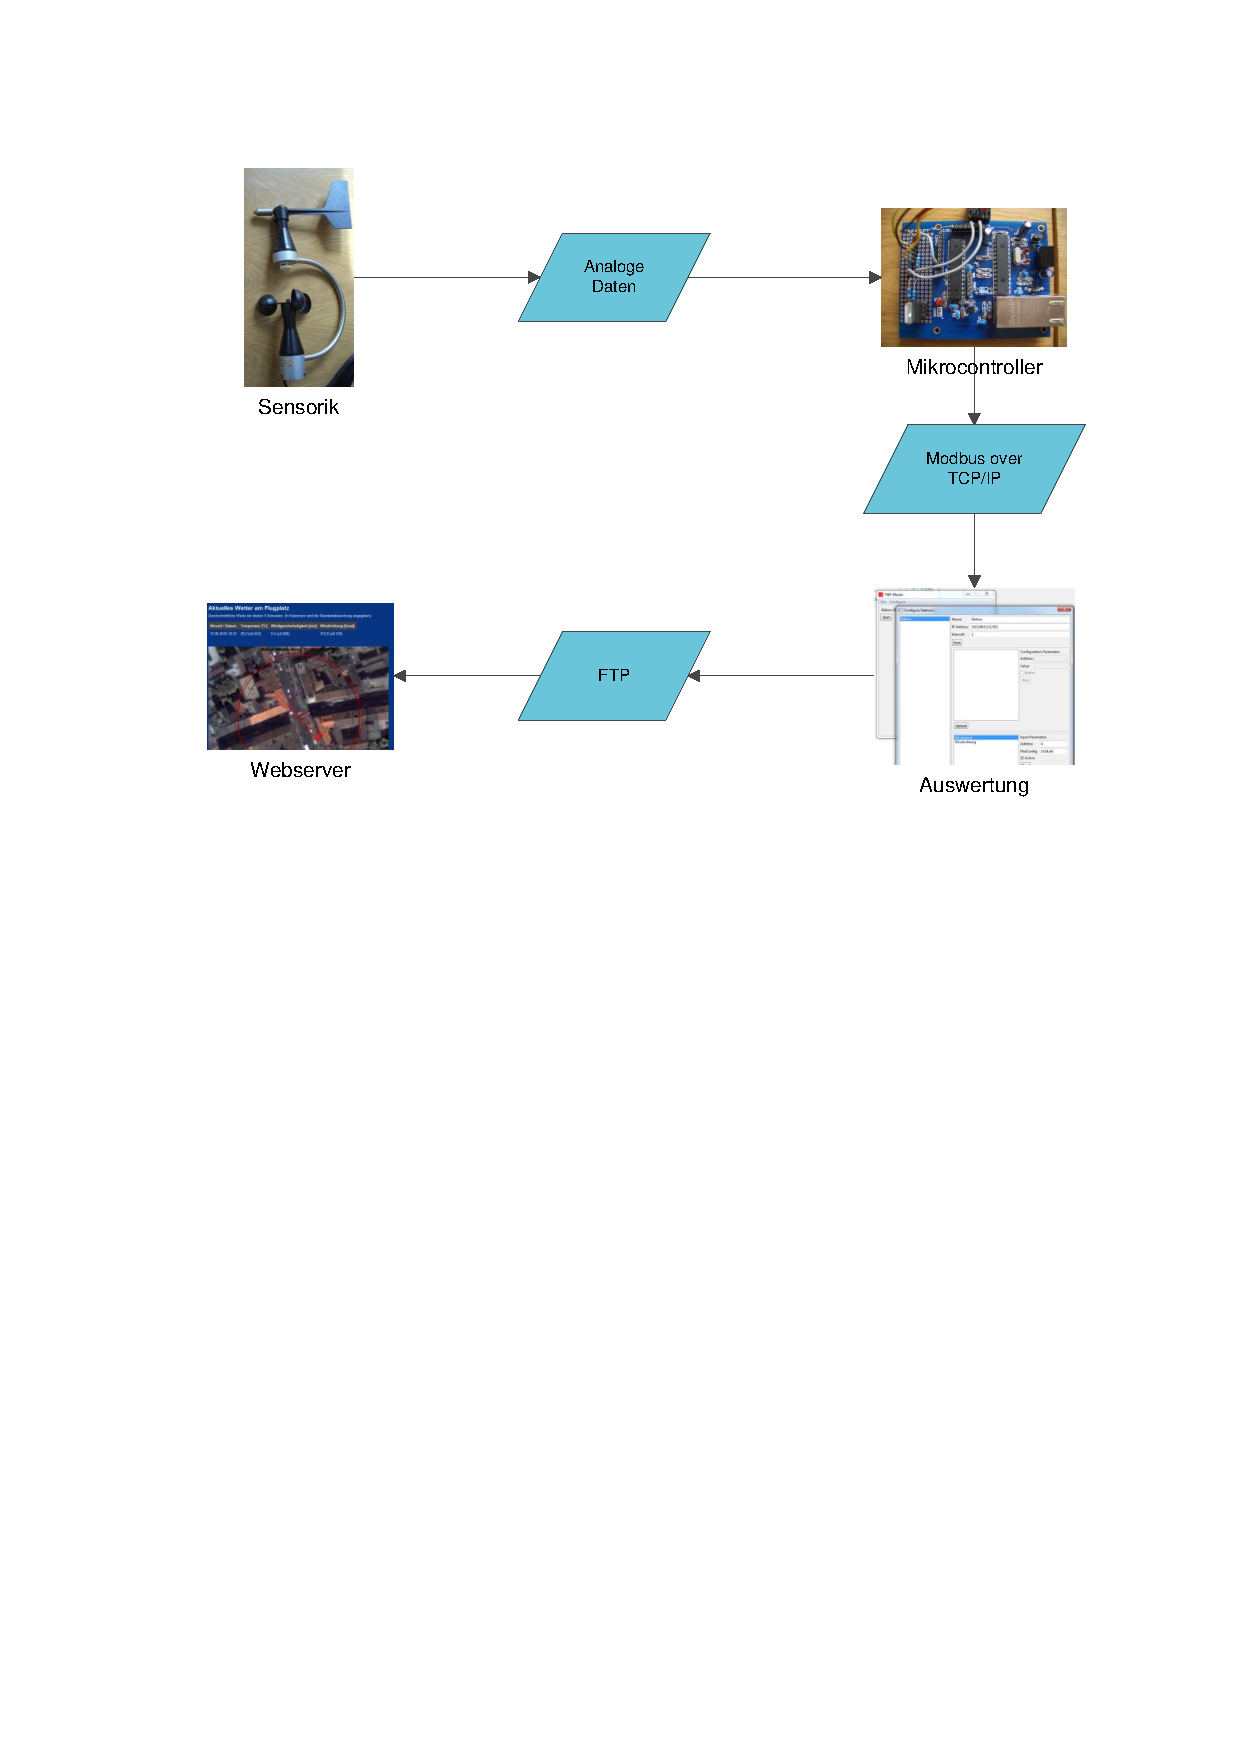
\includegraphics[width=\linewidth]{graphics/overview.pdf}
    \caption{Module and protocol overview of FWS}
    \label{fig:fws_overview}
\end{figure}

% section about_fws (end)